\documentclass[12pt]{article}



\usepackage{showlabels}
\usepackage{fullpage}
\usepackage{pslatex}
%\usepackage{latexsym}
\usepackage[english]{babel}
\usepackage[utf8]{inputenc}
\usepackage{amsmath}
\usepackage{bm}
\usepackage{graphicx}
\usepackage{tikz}
\usepackage{xcolor}
\usepackage{url}
%\usepackage[colorinlistoftodos]{todonotes}
\usepackage{rotating}
\usepackage{amssymb}

\usepackage{tikz-dependency}
\usepackage{longtable}


\newcommand{\R}[0]{\mathbb{R}}
\newcommand{\E}[0]{\mathbb{E}}
\newcommand{\Ff}[0]{\mathcal{F}}

\usepackage{multirow}

\newcommand{\soft}[1]{}
\newcommand{\nopreview}[1]{}
\newcommand\comment[1]{{\color{red}#1}}

\usepackage{amsthm}

\newcommand{\thetad}[0]{{\theta_d}}
\newcommand{\thetal}[0]{{\theta_{LM}}}

\newcounter{theorem}
\newtheorem{proposition}[theorem]{Proposition}
\newtheorem{thm}[theorem]{Theorem}
\newtheorem{corollary}[theorem]{Corollary}
\newtheorem{question}[theorem]{Question}
\newtheorem{example}[theorem]{Example}
\newtheorem{lemma}[theorem]{Lemma}

\definecolor{Red}{RGB}{255,0,0}
\newcommand{\red}[1]{\textcolor{Red}{#1}}
\newcommand{\jd}[1]{\textcolor{Red}{[jd: #1]}} 
\newcommand{\mhahn}[1]{\textcolor{Red}{[mhahn: #1]}} 
\newcommand{\rljf}[1]{\textcolor{Red}{[rljf: #1]}} 

\frenchspacing

\title{The Structure of Human Language Reflects Limitations of Working Memory}
\author{Michael Hahn, Judith Degen, Richard Futrell}
\date{2019}


\usepackage{scicite}

\usepackage{times}


\topmargin 0.0cm
\oddsidemargin 0.2cm
\textwidth 16cm 
\textheight 21cm
\footskip 1.0cm



\newenvironment{sciabstract}{%
\begin{quote} \bf}
{\end{quote}}



\date{}



%%%%%%%%%%%%%%%%% END OF PREAMBLE %%%%%%%%%%%%%%%%







\begin{document}

\baselineskip24pt


\maketitle

\begin{abstract}
  %  the Nature template:
  % 1-2 sentences basic introduction, for anyone
  Each of the roughly 6000 natural languages currently spoken in the world embodies a different system for encoding thoughts into linear strings of words.
  By characterizing the commonalities and differences among these systems we can gain insight into the cognitive machinery that underpins this fundamental aspect of human intelligence. 
  % 2-3 sentences detailed background, for scientists in related disciplines (linguistics, cogsci, computer science, info theory)
  In linguistics and cognitive science, there have been two \jd{unfinished sentence}

  % 1 sentence general problem
  % 1 sentence here we show
  Here we show that the order of words across human languages is structured to enable efficient transfer of information under the constraint that language must be comprehended and produced by agents with limited short-term memory capacities.
  We directly show that languages are optimized to minimize memory usage by calculating lower bounds on the amount of memory resources required for language comprehension in TODO \jd{random TODO} real languages and in random baseline languages, finding that the real languages require less memory.
  % 2-3 sentences how main result adds to knowledge
  Using concepts from information theory, we prove a theorem showing that any efficient communication system operating under memory constraints will exhibit a property called information locality: symbols which predict each other should be produced close to each other in time.
  We show that information locality subsumes several principles of word order previously proposed in the linguistics and cognitive science literature, and explains a number of the previously-documented universal patterns in word order across languages.    
	% TODO i'm wondering whether we should first mention the big result, and then say, well it also subsumes previously proposed constraints.
  % 1-2 sentences general context
  
  % 2-3 sentences broader perspective
  Our results suggest a view of natural language as a maximally efficient code for communication, subject to the particular information-processing constraints of the human mind. 
\end{abstract}

%Since short-term memory of this kind is known to be highly limited in capacity \cite{miller1956magical}, it makes sense for these capacity limits to comprise a major constraint on production and comprehension.



%The manuscript should start with a brief introduction describing the paper’s significance.
%The introduction should provide sufficient background information to make the article intelligible to readers in other disciplines, and sufficient context that the significance of the experimental findings is clear.
%Technical terms should be defined. Symbols, abbreviations, and acronyms should be defined the first time they are used.
%All tables and figures should be cited in numerical order. All data must be shown either in the main text or in the Supplementary Materials or must be available in an established database with accession details provided in the acknowledgements section. References to unpublished materials are not allowed to substantiate significant conclusions of the paper.

% introductory paragraph


Human languages express thoughts into sentences, i.e. linear strings of words. 
%For example, if your mountain climber friend Bob decided to turn back near the summit of Mt. Everest, you might say \emph{Bob gave the attempt to climb Mt. Everest up}.
% Run with this example
\jd{is the commented out example sth that will make it in? it does seem like an example would be good here}

Each language embodies a different strategy for encoding thoughts into strings of words. \jd{will this sentence and the next both survive?}

Languages differ considerably in the rules they apply to order information: English orders the object after the verb, Japanese places it before the verb.
Explaining the variation in the strategies languages use to  order underlying hierarchical structures into linear strings of words has been one of the foci of linguistic research (\jd{CITE}).
We show that these strategies reflect an underlying optimization principle: human languages are adapted to limitations in human working memory.

%We test the hypothesis that human languages represent different solutions to the problem of efficient computation with constrained working memory.
The suggestion that the structure of human language partly reflects a need for efficient processing under resource limitations has been present in the theoretical and functional linguistics literature for decades~\cite{berwick1984grammatical,hawkins1994performance};
however, it has been hard to test this idea without ad-hoc modeling assumptions. \jd{like what? why is the information-theoretic approach not subject to this ad-hoc-ness?}
%Alternative?: there has been debate about what shapes human language. role played by UG/innate constraints? environment? cognition?

We directly test the efficient processing hypothesis by applying a novel information-theoretic analysis to large-scale data from 54 languages, with expert annotations of underlying hierarchical structures~\cite{nivre-universal-2017}.

%%%%%%%%%%%%%%%%%%%%%%%%%%%%%%%%%%%


\begin{figure}
\centering
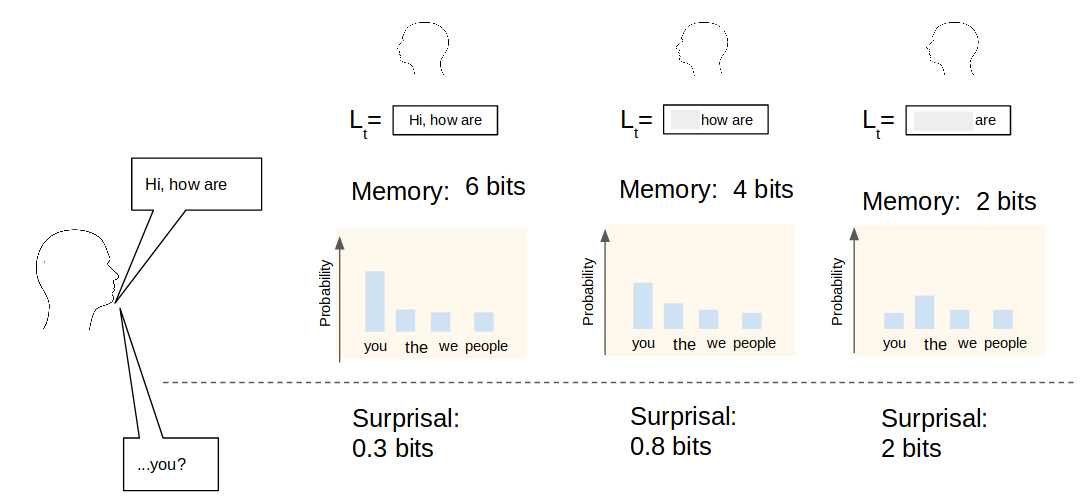
\includegraphics[width=0.9\textwidth]{figures-gdrive/communication.png}
	\caption{Memory and language comprehension. (1) A speaker produces a sequence of words. (2) A listener maintains a representation of the words received so far. The listener can represent these at higher (left) or lower (right) levels of precision. (3) Throughout communication, the listener generates probabilistic expectations about the next word. Higher precision of memory representations leads to more precise predictions. (4) When receiving the next word, the listener incurs surprisal depending on the predictions. Higher levels of fidelity in memory lead to lower surprisal on average. \jd{what do the numbers (1) (2) etc refer to? also: image is blurry, at least on my screen}}
	\label{fig:communication}
\end{figure}



We consider the process of language comprehension in a person processing a stream of words uttered by an interlocutor (Figure~\ref{fig:communication}).
Experimental research has established that such a listener (1) maintains information about the words received so far, and (2) forms probabilistic expectations about the upcoming words \jd{CITE}. %, and (3) words are easier to process when they are highly expected in context.
Importantly, the listener can represent the prior context at higher or lower levels of precision (Figure~\ref{fig:communication}).
More detailed memory representations lead to a higher working memory load, but also enable more precise predictions.
The psycholinguistic literature has established that humans differ in their capacity to store such representations \jd{CITE}, and that capacity limitations can create difficulties in language comprehension \jd{CITE}.

Experimental research has shown that human processing effort on a given word is strongly predicted by its surprisal, the degree to which it cannot be predicted from the preceding context \jd{CITE roger}.
Surprisal is known to be a strong linear predictor of processing effort as measured by per-word log-transformed reading times.
For an idealized listener with unbounded memory resources, surprisal will be given by the negative log-probability of a word given its preceding context:
\begin{equation}\label{eq:surp}
	-\log p(x_i|x_{1...i-1})
\end{equation}
where $x_i$ is the $i$-th word in a given utterance (or discourse).
%
%In reality, a listener will have bounded capacity to represent prior context.
A listener with limited memory of prior context will not be able to compute the full conditional distribution~(\ref{eq:surp}).
As in Figure~\ref{fig:communication}, we denote a listener's memory representation at time $t$ by $L_t$, which is some -- generally imperfect -- summary of the preceding context $\dots x_{t-3}x_{t-2}x_{t-1}$.
This listener will experience surprisal
\begin{equation}\label{eq:surp-listener}
	S :=	-\log p(x_t|L_t)
\end{equation}
upon hearing the next word $x_t$.
%The amount of information stored by the listener is the number of bits in $L_t$, i.e., its entropy $M := H[L_t]$.
%For a listener who invests less bits into representing information $L_t$ about prior context, $L_t$ will be a more coarse-grained representation of past observations.
%Thus, the predictions made by such a listener will be on average less accurate, and such a listener will incur greater processing effort $S$.

Information theory, specifically the Data Processing Inequality, implies that the average surprisal $S$ will be higher for a listener who represents past input at lower levels of precision. \jd{include an additional sentence on the DPI?}
Consequently, there is a tradeoff between memory and surprisal:
A listener can achieve lower levels of processing effort at the expense of increased memory load.

%Formally, we quantify memory as the number of bits about prior input that a listener represents.


%We quantify memory as the number of bits about prior input that a listener represents.
We prove a theorem describing how the shape of this tradeoff relates to language structure. %relating memory to the experienced comprehension difficulty $S$.
%Informally, the theorem says that languages support more efficient tradeoffs between short-term memory and comprehension difficulty when words are strongly predictive of their neighboring words.
This theorem captures formally that languages support more efficient tradeoffs between short-term memory and comprehension difficulty when words are strongly predictive of their neighboring words.


\begin{figure}
	(a)
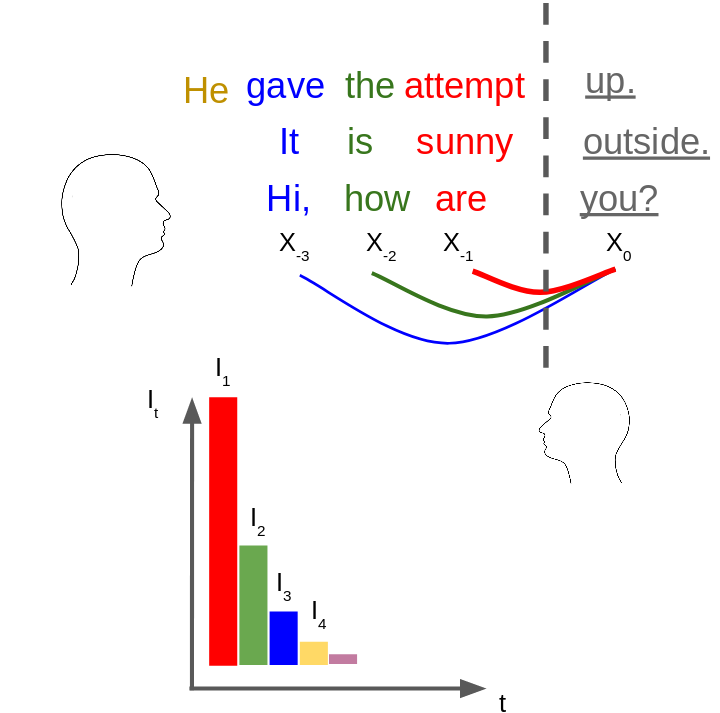
\includegraphics[width=0.4\textwidth]{figures-gdrive/mi-distance.png}
	(b)
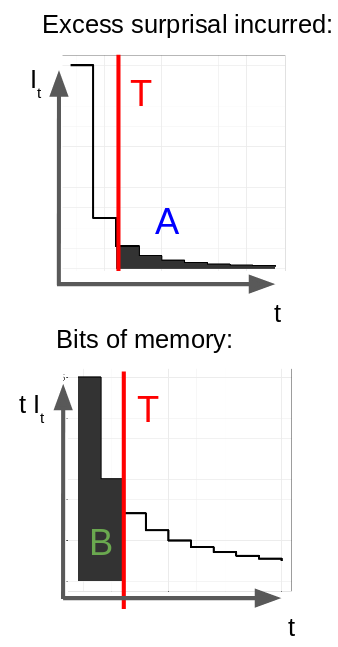
\includegraphics[width=0.2\textwidth]{figures-gdrive/theorem.png}
	(c)
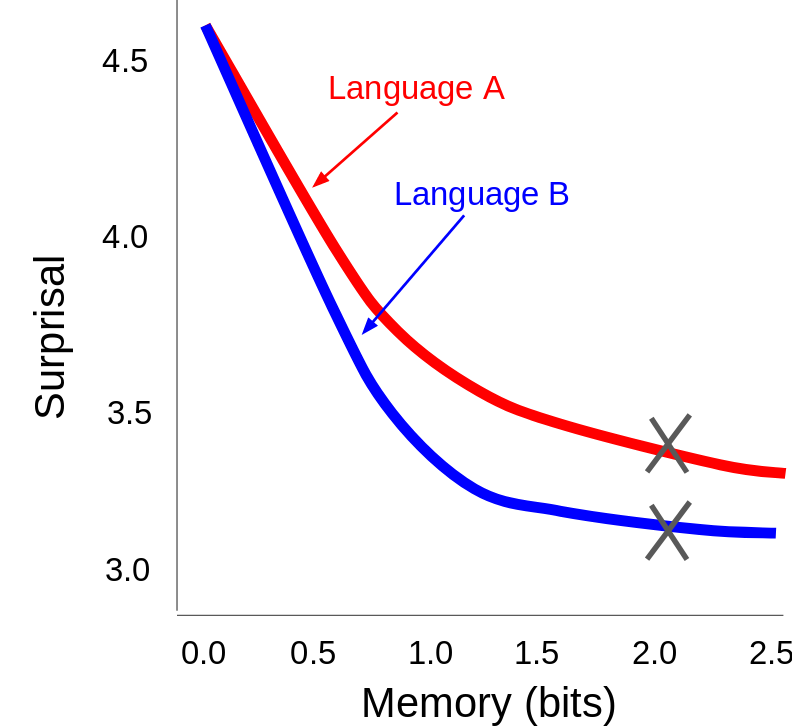
\includegraphics[width=0.2\textwidth]{figures-gdrive/tradeoff.png}
	\caption{
		(a) Conditional mutual information $I_t$ describes how much predictive information about the next word is provided, on average, by the word $t$ steps in the past.
		(b) Theoretical result: We plot $I_t$ (top) and $tI_t$ (bottom) as functions of $t$. A listener using $B$ bits memory (bottom) to represent prior observations will incur at least $A$ bits of extra surprisal beyond the entropy rate (top).
		(c) \jd{FILL OUT}
}\label{fig:theorem}
\end{figure}


%TODO
Let $I_t$ be the Conditional Mutual Information of two words $X_0, X_t$ conditioned on the intervening words:
\begin{equation}
	\operatorname{I}_t := \operatorname{I}[X_t, X_0 | X_1, \dots, X_{t-1}] = \operatorname{H}[X_t|X_1, \dots, X_{t-1}] - \operatorname{H}[X_t|X_0, \dots, X_{t-1}] 
\end{equation}
This quantity, visualized in Figure~\ref{fig:theorem} (a), measures how much predictive information is provided by the next word $X_t$ by the word $t$ steps in the past.
It is a statistical property of the language, and can be estimated from large-scale text data.
Our theoretical results describe how the tradeoff between memory and comprehension difficulty relates to $I_t$ (Figure~\ref{fig:theorem} (b)):
Consider a listener who invests $B$ bits of memory into representing past input.
We then consider the smallest $T$ such that the area under the curve of $t I_t$, to the left of $T$, has size $B$.
Such a listener will experience average surprisal at least $H[X_t| X_{<t}] + \sum_{t=T+1}^\infty I_t$.
By tracing out all values $T >0$, one can obtain a bound on the tradeoff curve for any possible listener.


An immediate consequence of this theoretical result is a general relation between memory and locality:
A language will enable more efficient tradeoffs if $I_t$ decays very fast as $t$ grows, which corresponds to strong concentration of predictive information in the recent past.

%We prove that, for any integer $T > 0$, a listener encoding $\sum_{t=1}^T t I_t$ bits of memory will incur average surprisal at least $H[X_t| X_{<t}] + \sum_{t=T+1}^\infty I_t$.
%maybe multiple sentences in def of It?
%define math, AND give people intuition.





\begin{figure}
\centering
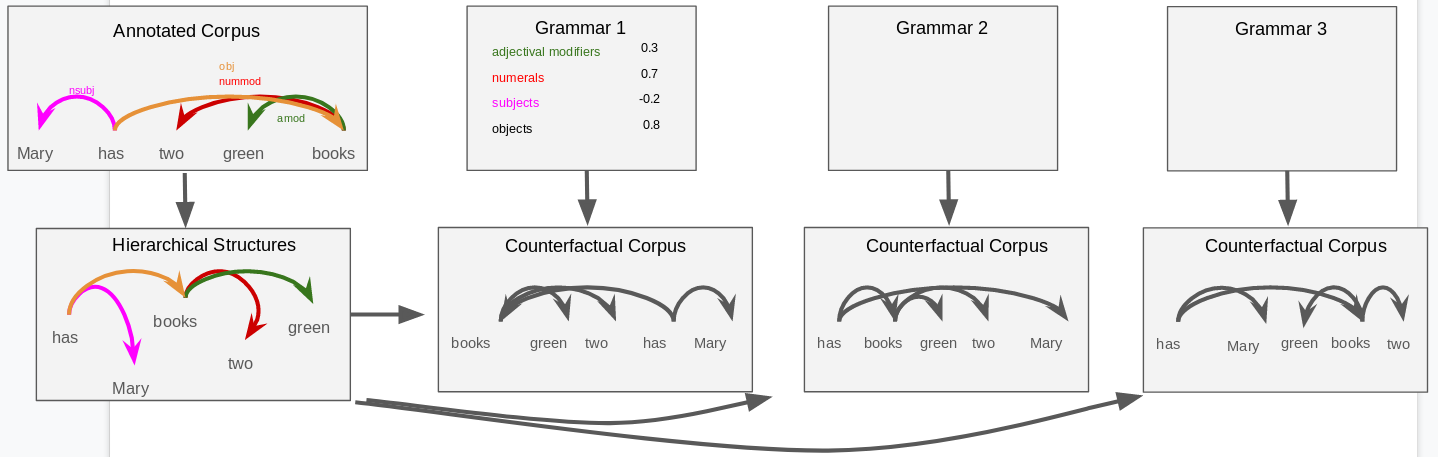
\includegraphics[width=\textwidth]{figures-gdrive/counterfactual-languages.png}
	\caption{Estimating chance by constructing counterfactual grammars and languages.\jd{this figure is again blurry for me. also looks like there's sth in the background on the left?}}\label{fig:grammars}
\end{figure}





Based on our theoretical result, we estimated the memory-surprisal tradeoff for 54 human languages, using standard estimation methods for language modeling based on neural networks~\cite{hochreiter-long-1997}.
We compared these against chance, that is, to tradeoffs that would be expected for languages that apply consistent grammatical rules as human language does, but have no bias towards any kind of processing efficiency or robustness.
For each language, we constructed counterfactual versions that differ from real languages in their word order, holding all other properties constant.
These counterfactual versions use randomly created grammars for linearizing hierarchical structures into sentences (see Figure~\ref{fig:grammars}), akin to those found in human languages. \jd{refer to SI here and make sure to include a lot more information in the SI about how the grammars were created}
%These random grammars apply consistent grammatical rules as human language does, but have no bias towards any kind of processing efficiency or robustness.


%\begin{figure}
%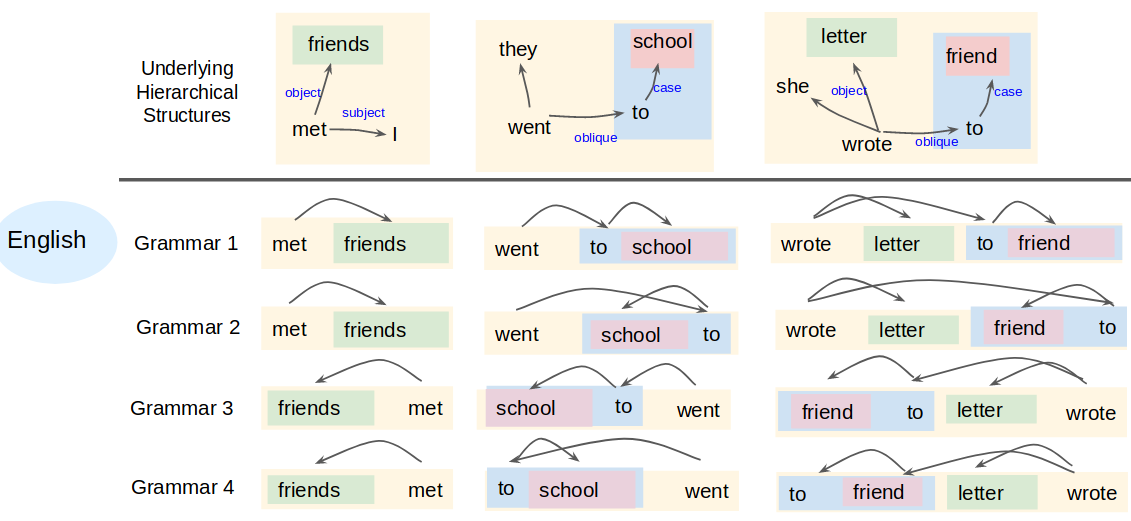
\includegraphics[width=\textwidth]{figures/grammars.png}
%	\caption{Grammars specify the rules by which languages linearize underlying hierarchical structures into strings of words. In this example, the first grammar corresponds to English; the others are counterfactual. (\textbf{TODO} this draft is currently just copied from the Greenberg Universals paper, probably have to make it look a bit different. Also, adapt it so it looks more like `hierarchical structure' than `dependency graphs'. And add subjects.) }\label{fig:grammars}
%\end{figure}
%


Results are shown in Figure~\ref{fig:results}.
Human languages lead to a more efficient tradeoff than expected by chance ($p < 0.0001$).
We replicated this result with different methods of estimating chance (see SI).

At extremely low memory capacities, real and baseline languages are equally efficient.
However, the curves soon diverge, and real language provides a more efficient tradeoff.
The point of divergence is given by that memory capacity that fully exhausts information provided by the immediately preceding word, that is, when the capacity of a Markov model in approximating language is exhausted.


\begin{figure}
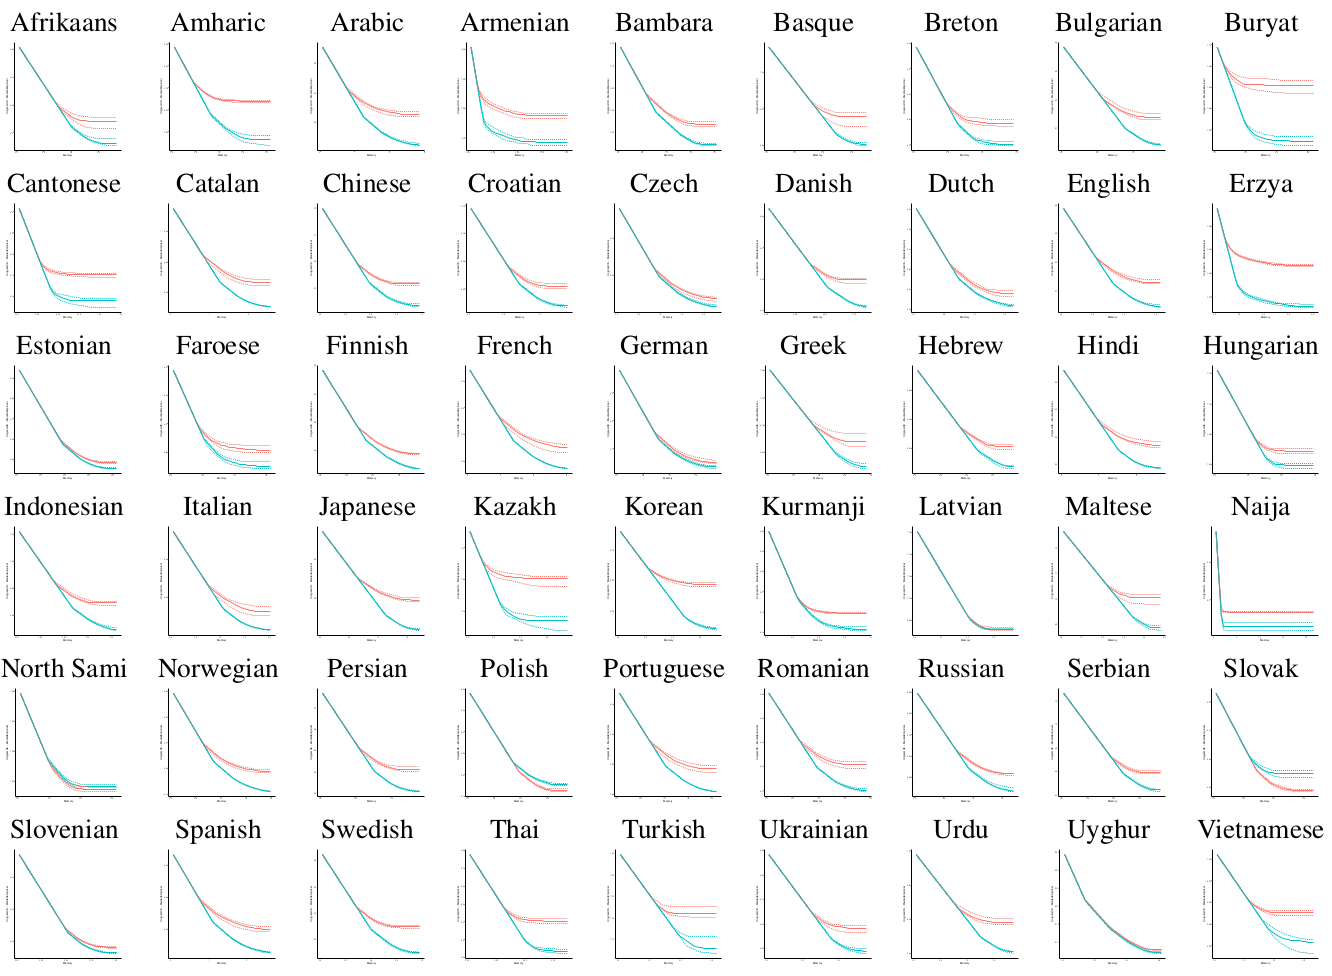
\includegraphics[width=\textwidth]{figures/full-results.png}
	\caption{\jd{FILL OUT; make less blurry}}\label{fig:results}
\end{figure}


say s.th. about estimates of human working memory. only if the last word is the only thing do things not make a difference.


Things to perhaps mention:

%- Potentially cite \cite{PhysRevLett.115.098701} as a reference saying that physical systems have bounded memory?

- Computational efficiency has been mentioned in mainstream syntax, though it's not so clear what it means there \cite{chomsky2005three,hauser2002faculty}.

- Beyond human language, our theoretical result applies to other stochastic processes. To the extent that they may be affected by bounded memory in computation, we predict they should also enable efficient tradeoffs between memory and surprisal.

- Our results provide a new perspective on several previous results: (1) DLM, (2) DLT, (3) decay of MI over distance.






%
%-This listener will represent information about past words in their short-term memory.
%We quantify the amount of memory resources that are used by the number of bits.
%We consider the question of how many bits of information this listener has to carry from one instant to the next.  %\jd{why?}
%
%-Human language is well known to have a large amount of context-dependence in the meanings and forms of words.
%Understanding what a word means often requires consideration of context. 
%Consider the sentence `The climber gave the attempt to reach the peak up.'
%Understanding the word \emph{up} requires establishing that it is related to the word \emph{gave} -- neither of them has the meaning of `give up' by itself.
%In order to understand this sentence correctly, a listener has to store some information about the occurrence of the word \emph{gave} until reaching \emph{up}.
%For language comprehension, this means that a listener's ease of comprehension will be modulated by how much memory they invest into representing information about past context:
%A listener who remembers more of the past context should have less difficulty understanding, at the cost of increased working memory load. 
%We thus expect there to be a tradeoff between a listener's ease of language understanding and their working memory load.
%


%
%For example, 
%- discontinuous idioms
%- example? something like `John threw the trash out'
%- particle verb, with completely idiomatic meaning. `give up' `the climber gave the attempt to reach the peak of Mount Everest up' could have figure `he gave the attempt to sculpture out of marble up'. understanding what the word means in contet requires understanding of the past.
%- something with a relative clause `The child that was playing on the street had a red ball' -- should not forget the `child'.
%- center embedding: `The physician who consulted the cardiologist checked the files in her office' -- (Fedorenko, Gibson, and Rohde (2006))
%Make clear that Understanding requires knowing the past. (introduce prediction earlier?) Example? Then formally introduce prediction.

%A maximally efficient listener will incur surprisal exactly at the entropy rate of the language, i.e., at the rate at which the language provides information.


%We use information theory to quantify the tradeoff between memory load and ease of understanding.
%This quantity is known to be a strong linear predictor of human processing effort.

%- can refer to general things such as Friston
%TODO Make sure letters are intutive.

%Since $L_t$ is some summary representation, 
%Therefore, ne should expect that processing effort $S$ increases for a listener who invests less bits into representing information about prior context.\jd{why? this is important.}

%For instance, in `The climber gave the attempt to reach the peak up', the word \emph{up} is less surprising to a listener who has maintained some information about the word \emph{gave} in their memory.


% from the introduction to paper.tex:
%Since the 1950s, it has been a persistent suggestion that human language processing is shaped by a resource bottleneck in short-term memory.
%Language is produced and comprehended incrementally in a way that crucially requires both speaker and listener to use an active memory store to keep track of what was previously said.
%Since short-term memory of this kind is known to be highly limited in capacity \cite{miller1956magical}, it makes sense for these capacity limits to comprise a major constraint on production and comprehension.
%Indeed, a great deal of work in sentence processing has focused on characterizing the effects of memory constraints on language processing \cite{gibson-linguistic-1998,lewis-activation-based-2005,levy2013memory}.
%
%At the same time, the field of functional linguistics has argued that these resource constraints not only affect online language processing, they also shape the form of human language itself.
%For example, the Performace--Grammar Correspondence Hypothesis (PGCH) of \citet{hawkins1994performance} holds that forms which are practically easier to produce and comprehend end up becoming part of the grammars of languages, and that this process can explain several of the universal properties of human languages originally documented by \citet{greenberg-universals-1963}.
%
%Here we take up the question of how to characterize short-term memory capacity limitations in language processing for both speakers and listeners, and the question of whether natural language grammars are shaped by these limitations.
%Whereas previous theories were based on specific mechanistic models of memory, our theory is purely information-theoretic, meaning that our predictions will hold independently across a wide variety of implementations and architectures.
%
%Our main new concept is the idea of a \emph{memory--surprisal tradeoff}: it is possible for a listener to achieve greater ease of word-by-word comprehension at the cost of investing more computational resources into remembering previous words, and the particular shape of the resulting tradeoff of depends on the word order properties of a language. Analogous results also hold for language production by resource-constrained speakers. We show evidence that the preferred word orders of natural languages are those that enable efficient memory--surprisal tradeoffs.
%
%



%However, testing this hypothesis has been difficult for two reasons:
%First, this requires a large amount of data representing the distribution of underlying hierarchical structures that people communicate,
%and
%second, because this presupposes a computatioal model of processing efficiency.
%Large-scale data has recently become available in the form of corpora annotated with underlying hierarchical structures across dozens of languages~\cite{nivre-universal-2017}.

%We test the idea that language is optimized for processing with limited resources, in particular with limited memory resources.


%Let $I_t$ be the Conditional Mutual Information of two words $X_0, X_t$ conditioned on the intervening words:
%\begin{equation}
%I_t := I[X_t, X_0 | X_1, ..., X_{t-1}] = H[X_t|X_1, ..., X_{t-1}] - H[X_t|X_0, ..., X_{t-1}] 
%\end{equation}
%We prove that, for any integer $T > 0$, a listener encoding $\sum_{t=1}^T t I_t$ bits of memory will incur average surprisal at least $H[X_t| X_{<t}] + \sum_{t=T+1}^\infty I_t$.



%
%Memory refers to information about previous parts of a sentence maintained in short-term memory.
%While memory limitations have been shown experimentally to affect human language processing, there is no consensus on the architecture used to represent memories.
%
%Here, for the first time, we provide an information-theoretic integration of these two aspects of processing, leading to a general theory of the computational efficiency of language.
%
%We denote a listener's memory representation at time $t$ by $L_t$, which is some -- generally imperfect -- summary of the context $X_{<t}$.
%This listener will experience surprisal
%\begin{equation}
%	S :=	-\log P(X_t|L_t)
%\end{equation}
%upon hearing the next word.
%%We quantify memory as the number of bits about prior input that a listener represents.
%The minimal amount of information stored is the number of bits in $L_t$, i.e., its entropy $M := H[L_t]$.
%%related to work in physics on the ability of physical systems to represent memory, representing more bits costs more memory \cite{PhysRevLett.115.098701}
%We note that there is a tradeoff between average memory, $\E[S]$ and memory $H[L_t]$: A listener who invests more memory resources to create representations of the past will incur lower average surprisal.
%
%We predict that languages order information in such a way as to create an optimal tradeoff.

%We study language as a 




%Data for (1) has become available with UD, and there is Richard's 2015 paper and other DLM work, but the relation between what they investigate (DLM) and processing is only heuristic.
%futrell2015largescale

%We use information-theory to for the first time really test (2).
%We use information-theoretical lower bounds on the difficulty in language processing.


\bibliographystyle{Science}

\bibliography{literature}

%
%
%\begin{figure}
%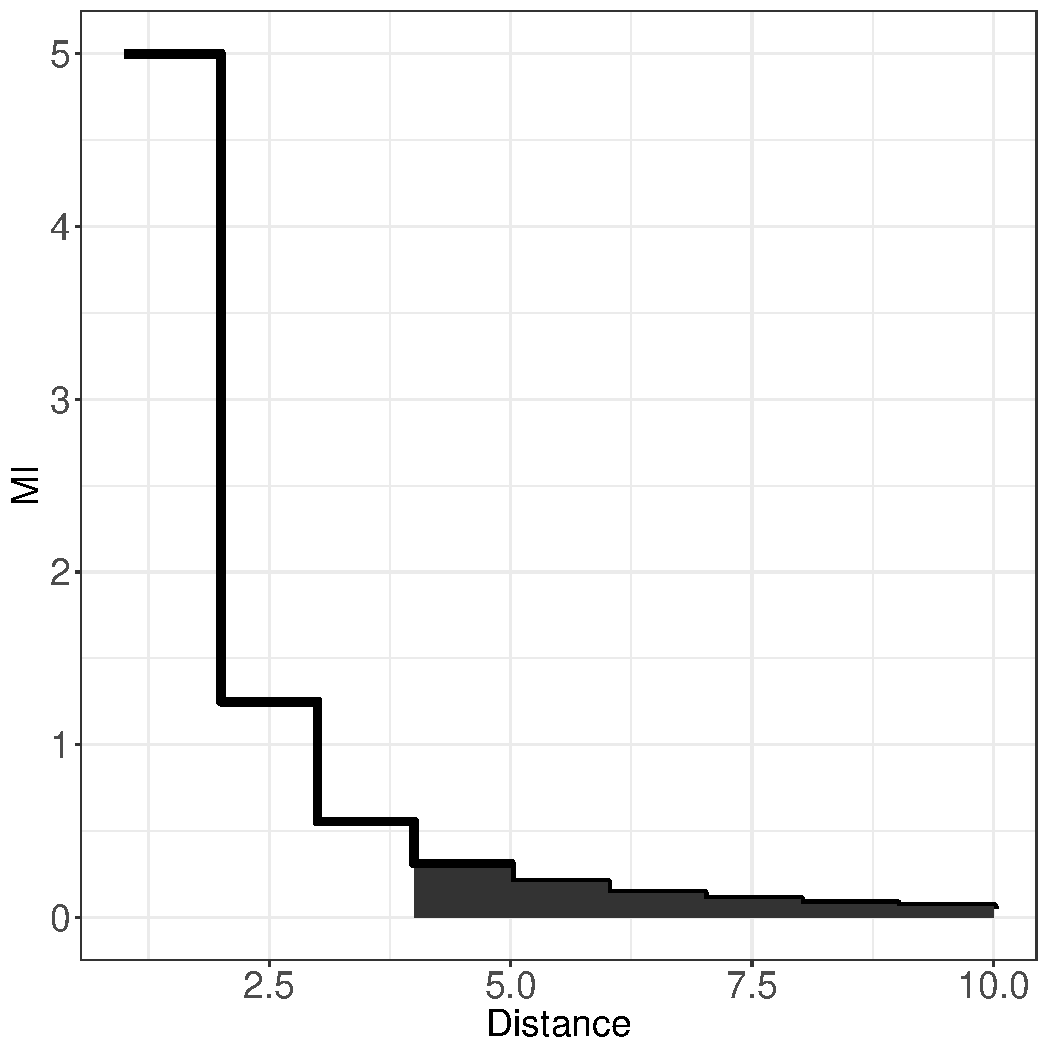
\includegraphics[width=0.45\textwidth]{toy/add-surp.pdf}
%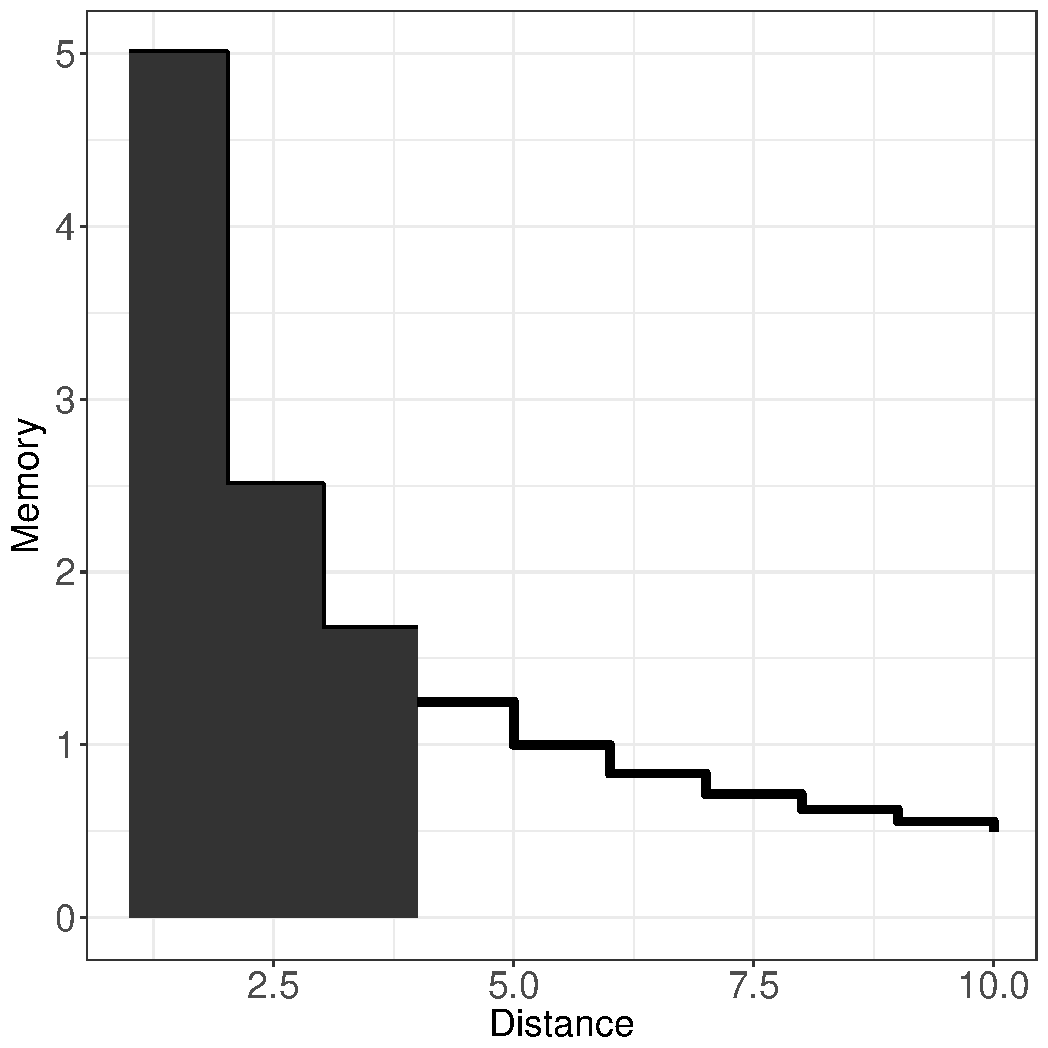
\includegraphics[width=0.45\textwidth]{toy/lower-mem.pdf}
%	\caption{Illustration for Proposition~\ref{prop:suboptimal}. Listeners can trade off memory and surprisal: A listener only investing memory of the amount given by the black area on the right will incur at least the black area on the left in additional surprisal. In the given example, $T=4$. By varying $T$, the two areas describe the listener's memory-surprisal tradeoff curve.}\label{fig:listener-tradeoff-decay}
%\end{figure}
%

%(up to ~2500 words including references, notes and captions
% abstract
% introductory paragraph
%up to four figures or tables
%about 30 references


\appendix{SI}


\section{Materials and Methods}

\subsection{Experimental Design}
\subsection{Statistical Analysis}





\end{document}


